\documentclass[letterpaper,11pt]{article}
\oddsidemargin -1.0cm \textwidth 17.5cm

\usepackage[utf8]{inputenc}
\usepackage[activeacute,spanish, es-lcroman]{babel}
\decimalpoint
\usepackage{amsfonts,setspace}
\usepackage{amsmath}
\usepackage{amssymb, amsmath, amsthm}
\usepackage{comment}
\usepackage{float}
\usepackage{amssymb}
\usepackage{dsfont}
\usepackage{anysize}
\usepackage{multicol}
\usepackage{enumerate}
\usepackage{graphicx}
\usepackage[left=1.5cm,top=1.5cm,right=1.5cm, bottom=1.7cm]{geometry}
\setlength\headheight{1.5em} 
\usepackage{fancyhdr}
\usepackage{multicol}
\usepackage{hyperref}
\usepackage{wrapfig}
\usepackage{subcaption}
\usepackage{siunitx}
\usepackage{cancel}
\pagestyle{fancy}
\fancyhf{}
\renewcommand{\labelenumi}{\normalsize\bfseries P\arabic{enumi}.}
\renewcommand{\labelenumii}{\normalsize\bfseries (\alph{enumii})}
\renewcommand{\labelenumiii}{\normalsize\bfseries \roman{enumiii})}

\begin{document}

\fancyhead[L]{\itshape{Facultad de Ciencias F\'isicas y Matem\'aticas}}
\fancyhead[R]{\itshape{Universidad de Chile}}

\begin{minipage}{11.5cm}
    \begin{flushleft}
        \hspace*{-0.6cm}\textbf{FI1100 Introducción a la Física Moderna}
    \end{flushleft}
\end{minipage}

\begin{picture}(2,3)
    \put(366, -10){
\includegraphics[scale=0.9]{Imágenes/logo/dfi-fcfm.pdf}}
\end{picture}

\begin{center}
	\LARGE\textbf{Problemitas de MAS}
\end{center}

\vspace{-1cm}

\begin{enumerate}\setlength{\itemsep}{0.4cm}

\rfoot[]{pág. \thepage}

\item[]

\item Un bloque de masa $m$ se encuentra en un plato de masa $M$. Si el sistema es sostenido por un resorte ideal de constante elástica $k$ y largo natural $\ell_0$
\begin{enumerate}
    \item ¿Cuál es la posición de equilibrio del sistema?

    \item Asumiendo que el resorte se comprime una distancia $A$ desde el equilibrio, ¿cuál es la frecuencia vertical de oscilación?

    \item ¿Cuál es la amplitud máxima para que la masa $m$ no se despegue del plato en cualquier instante del movimiento?
\end{enumerate}

\begin{figure}[H]
    \centering
    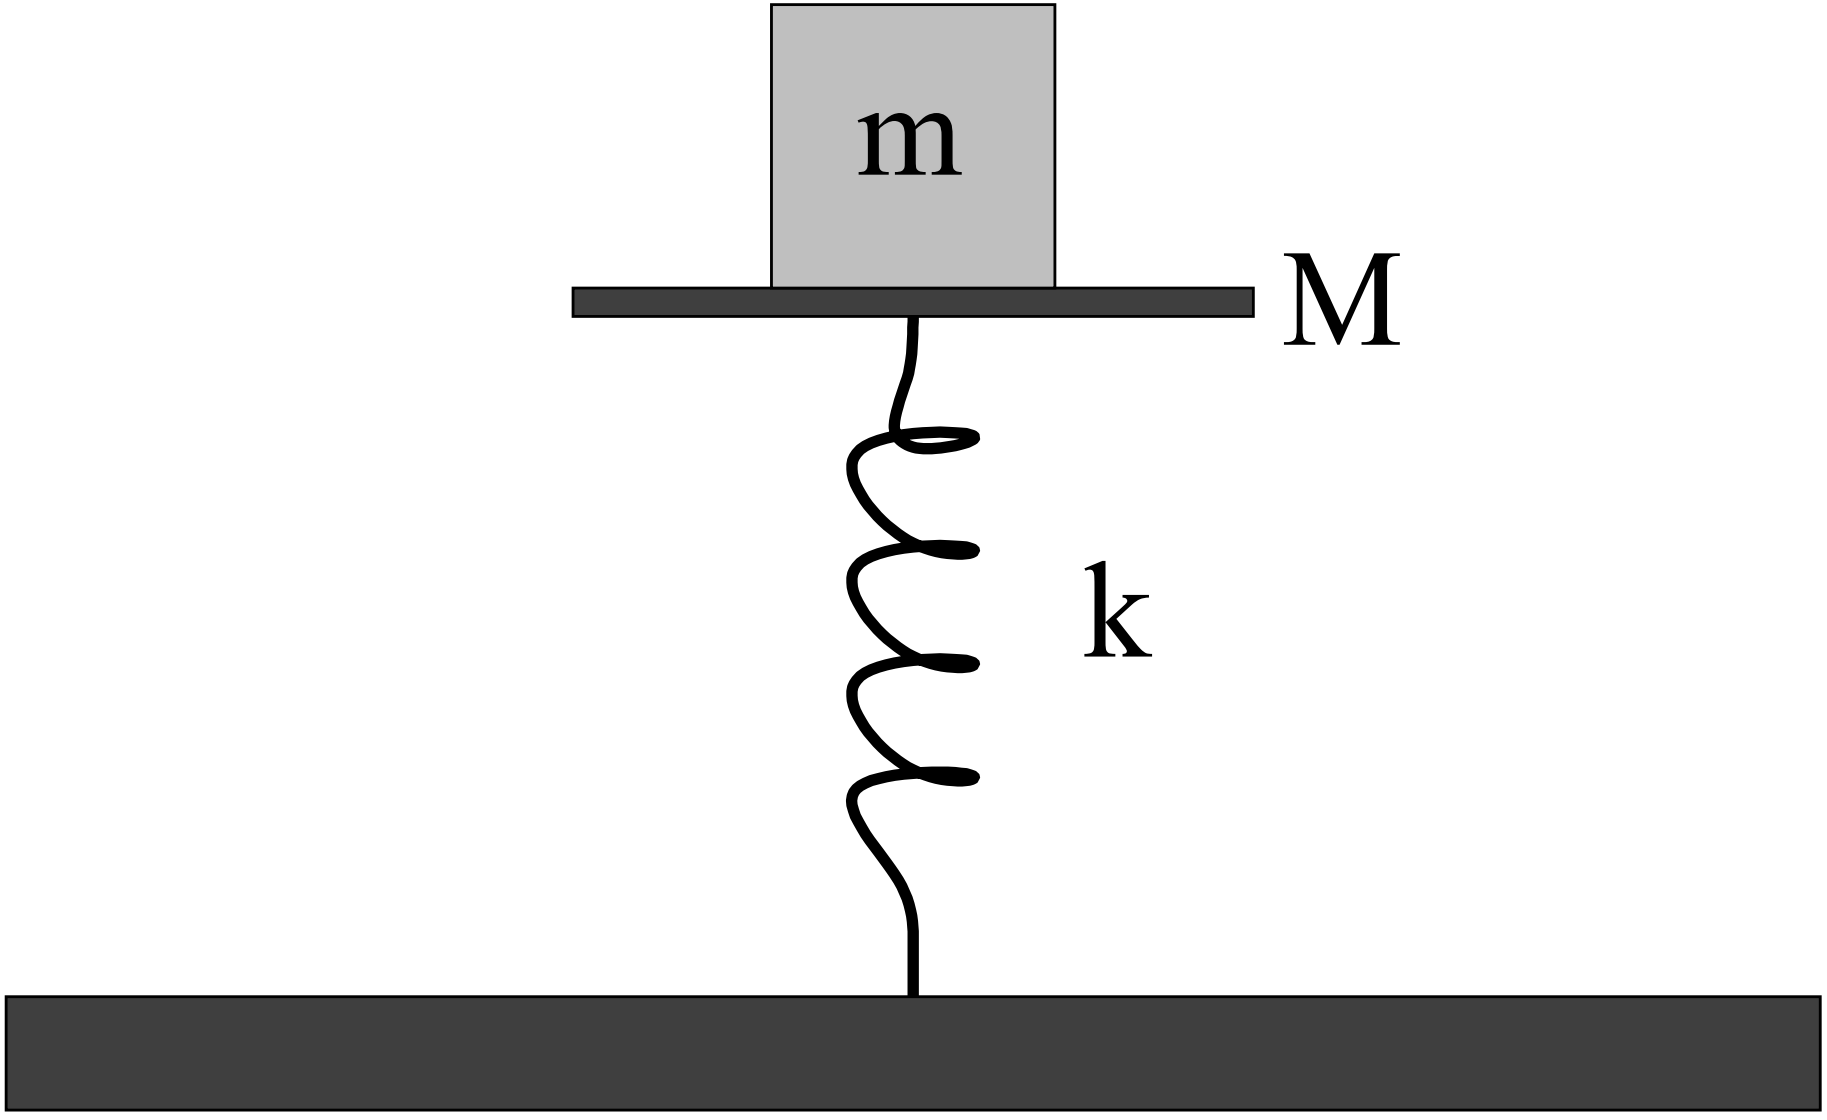
\includegraphics[width=0.3\linewidth]{Imágenes/clases/plato masa.png}
\end{figure}


\item Un bloque de masa $M$, en reposo sobre una mesa horizontal sin fricción, está unido a un soporte rígido por medio de un resorte de constante de fuerza $k$. Una bala de masa $m$ y velocidad $v$ golpea al bloque como se muestra en la figura. Si la bala se queda empotrada en el bloque, determine la amplitud del movimiento armónico simple resultante

\begin{figure}[H]
    \centering
    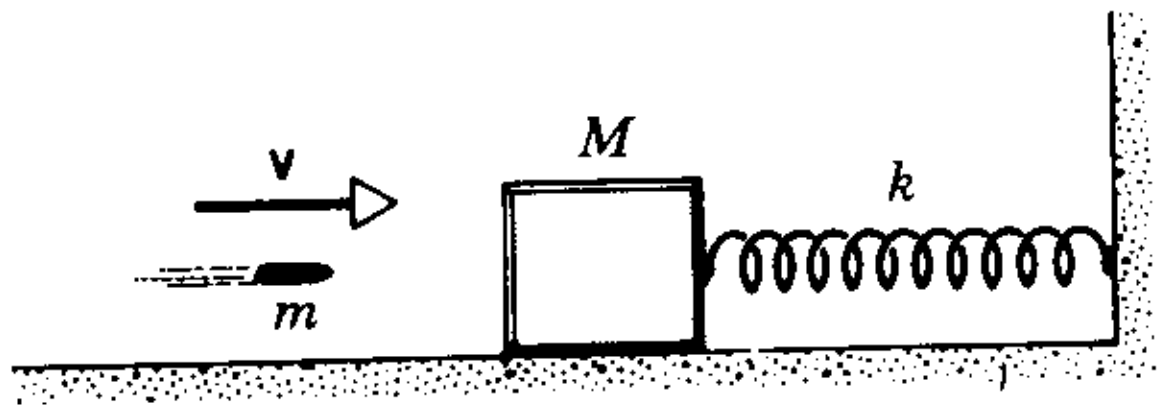
\includegraphics[width=0.3\linewidth]{Imágenes/clases/bala.png}
\end{figure}

\item \textbf{[P1-C1 2023-1]} Se tiene una masa $m$ sostenida de dos cuerdas de largos $L_1$ y $L_2$, con tensiones $T_1$ y $T_2$ respectivamente en presencia de gravedad, como se muestra en la figura. Considere que $T_2$ es conocido y $T_1$ es tal que el sistema no se mueve verticalmente.
Si inicialmente la masa se suelta desde el reposo a una distancia $x$

\begin{enumerate}
    \item Calcule el valor de $T_1$ para que el sistema no se mueva verticalmente
    \item Encuentre la frecuencia angular de oscilación
    \item Calcule el periodo de oscilación de la misma
    \item Calcule la amplitud de oscilación de la masa
\end{enumerate}

Considere para sus cálculos y aproximaciones $x\ll L_1, L_2$, y que las tensiones se mantienen al deformarse la cuerda

\begin{figure}[H]
    \centering
    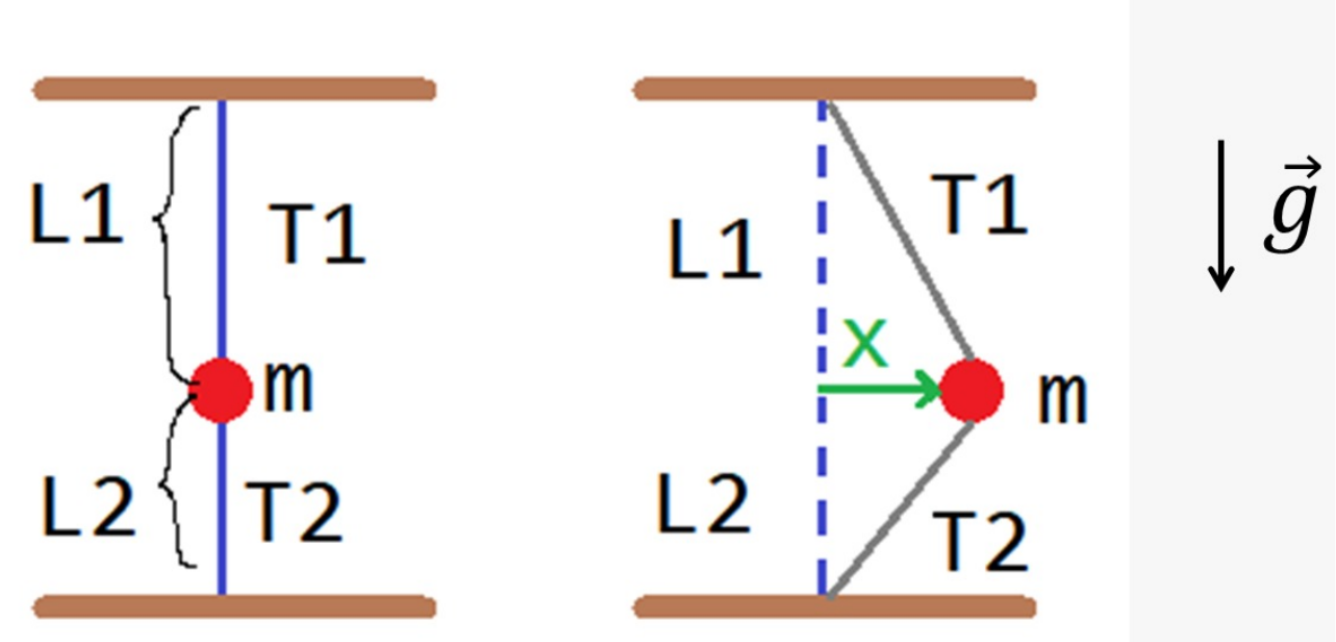
\includegraphics[width=0.3\linewidth]{Imágenes/clases/p1c3.png}
\end{figure}

\end{enumerate}
\end{document}